The proposed ECal trigger was simulated to test trigger cuts, verify
that the trigger has acceptable efficiency for A' events, and verify 
that the trigger rate is compatible with the HPS DAQ in all running conditions. 

The CEBAF beam bunch structure was simulated by sending one bunch 
equivalent of electrons, 
625 (1.1 GeV), 2,500 (2.2 GeV) and 5,625 $e^-$'s (6.6 GeV), through 
the target, and total 50 million bunches of beam backgrounds 
(equivalent to 100 ms of beam) were 
generated at each beam energy. The details of the target interactions are given in Section \ref{sec:backgrounds}.
Since the trident production process 
was not in EGS5, trident events were generated with MadGraph/MadEvent 
and overlaid on the beam background bunches with average rate 
expected from the trident cross section.
For the trigger acceptance studies, A' events were generated with 
MadGraph/MadEvent at 1.1, 2.2, and 6.6 GeV.

The complete chain of signal evolution in the ECal crystals and 
signal processing through the trigger system was simulated
by following closely the ECal trigger description in Section \ref{sec:triggerdaq}. 
Starting from the energy deposits in the ECal crystals, signals were 
generated using the CR-RC shaper function with a time constant of 15 ns
measured with the ECal crystals, amplitudes were sampled and pulse data 
evaluated every 4 ns (simulating FADC), and the cluster 
finding algorithm and trigger logic were applied (simulating CTP and SSP). 
The simulation has been tested against the actual performance of the test run detector and DAQ: see Section \ref{sec:ecalperformance}.

The trigger parameters described in Section \ref{sec:triggerdaq} are 
chosen by running the simulation and plotting the relevant variables 
for beam background and A' events. This is done for each beam energy 
and a set of A' masses for each beam energy. 
Figure \ref{fig:coplanarity} shows the coplanarity angle vs. the azimuthal 
angle of the lower-energy cluster, indicating that A' events 
tend to have small coplanarity angles. Figure \ref{fig:energy-distance} shows
the distance from beam axis vs. energy of the lower-energy cluster,
indicating that the energy-distance cut can reduce the beam background effectively.
Figure \ref{fig:ediff} shows the cluster energy difference vs. energy sum,
indicating that the energy sum cut can retain A' events effectively.       


These cuts are chosen to lie between the loosest reasonable values (accept as many A' events as possible) and the tightest (reject as many background events as possible). In some cases this leads to different cut values at different beam energies---for example, the coplanarity cut is looser at 1.1 GeV because the background events are clustered at large uncoplanarity and a relatively loose cut rejects most of them, but the cut is tighter at higher beam energies.

\begin{figure}[ht]
	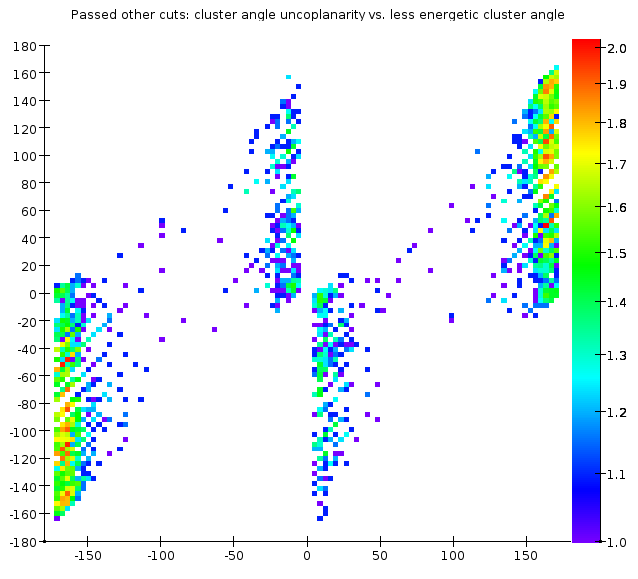
\includegraphics[width=0.45\textwidth]{performance/trigger/coplanarity_22}
	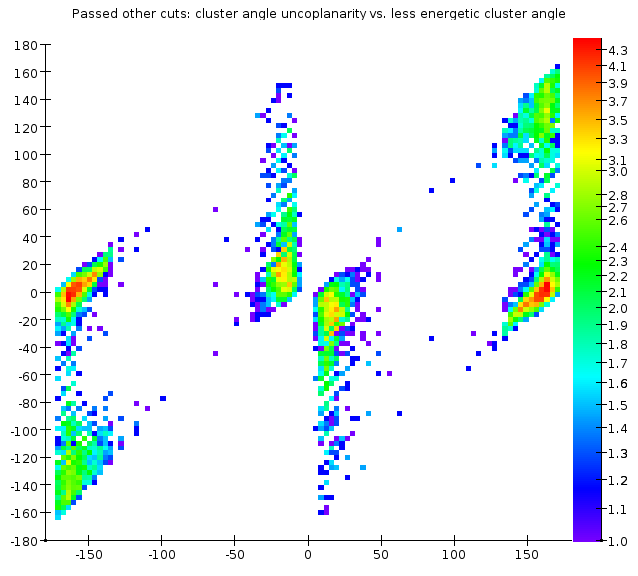
\includegraphics[width=0.45\textwidth]{performance/trigger/coplanarity_22_075mev}
	\caption{\small{Deviation of cluster pairs from coplanarity (units of degrees) for 2.2 GeV beam; background and 75 MeV A' tridents are shown. The X-axis is the azimuth around the beam axis ($\phi_1$) of the lower-energy cluster, such that 0 degrees is the positron side of the detector and 180 degrees is the electron side; the Y-axis is the difference between the azimuth angles ($\phi_1-\phi_2 - 180$) of the two clusters. The coplanarity cut's acceptance region is the space between the red lines.}}
	\label{fig:coplanarity}
\end{figure}

\begin{figure}[ht]
	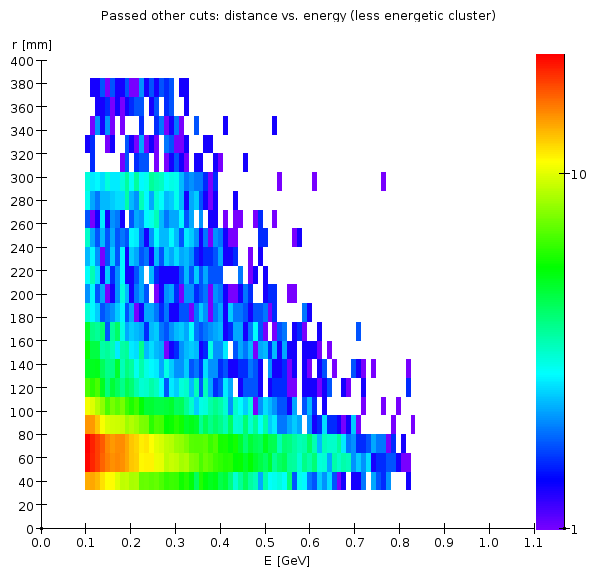
\includegraphics[width=0.45\textwidth]{performance/trigger/energy-distance_22}
	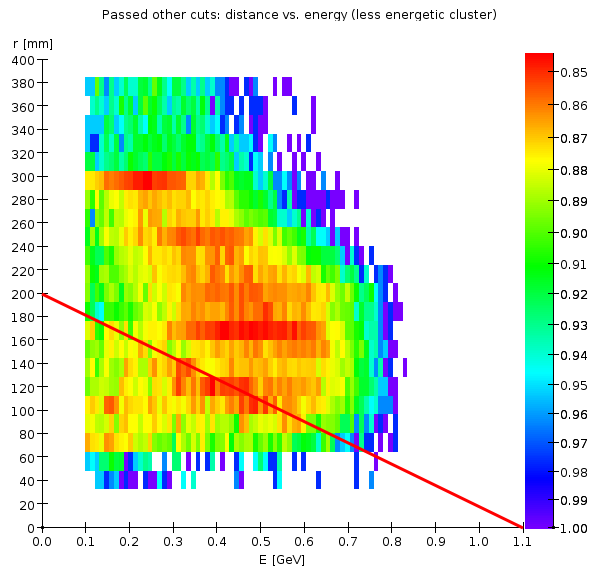
\includegraphics[width=0.45\textwidth]{performance/trigger/energy-distance_22_075mev}
	\caption{\small{Energy and distance from beam axis of the lower-energy cluster, for 2.2 GeV beam; background and 75 MeV A' tridents are shown. The energy-distance cut's acceptance region is above the red line.}}
	\label{fig:energy-distance}
\end{figure}

\begin{figure}[ht]
	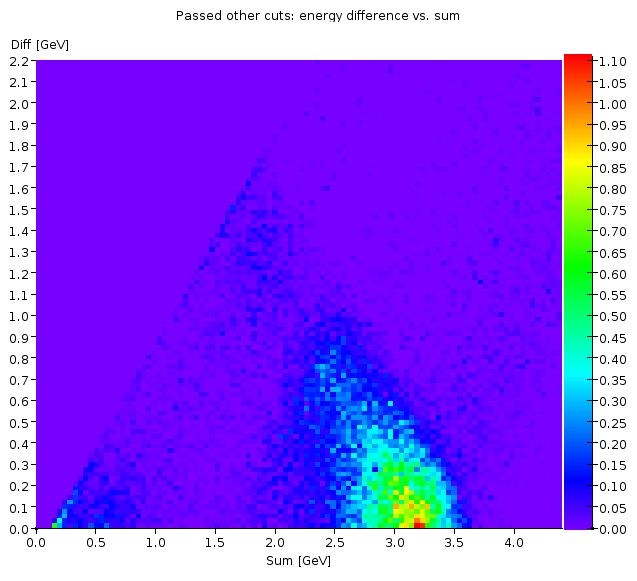
\includegraphics[width=0.45\textwidth]{performance/trigger/ediff_22}
	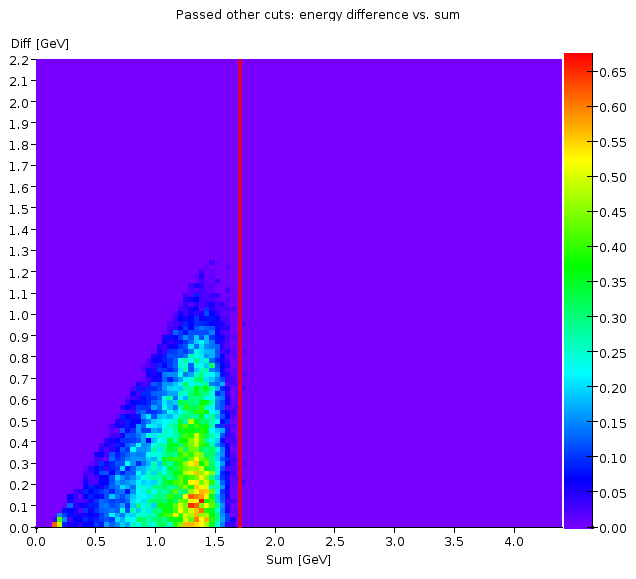
\includegraphics[width=0.45\textwidth]{performance/trigger/ediff_22_075mev}
	\caption{\small{Energy sum and difference of cluster pairs, for 2.2 GeV beam; background and 75 MeV A' tridents are shown. The energy difference cut's acceptance region is left of the red line.}}
	\label{fig:ediff}
\end{figure}

The following trigger parameters were determined to be independent of beam energy:
\begin{itemize}
	\item Minimum cluster energy ($E_{min}$): 0.1 GeV
	\item Distance ($r_{edist}$) in the energy-distance cut: 200 mm
	\item Energy ($E_{edist}$) in the energy-distance cut: $0.5\times E_{beam}$
\end{itemize}

Table \ref{tab:trigcuts} summarizes the trigger parameters that were found dependent on the beam energy. 
The remaining trigger parameters given in Section \ref{sec:triggerdaq} did not have a significant 
effect on specificity of the trigger.

\begin{table}
	\begin{tabular}{|l|r|r|r|}
		\hline
		Beam energy [GeV] & $E_{max}$ [GeV] & $Esum_{max}$ [GeV] & $\Delta\phi_{max}$ [$^\circ$] \\
		\hline
		1.1	&	0.7	&	0.8	&	90\\
		2.2	&	1.6	&	1.7	&	45\\
		6.6	&	5.0	&	5.5	&	60\\
		\hline
	\end{tabular}
	\caption{ {\small Trigger parameters optimized for different beam energies.}
	\label{tab:trigcuts}}
\end{table}

Trigger rates are shown in Table \ref{tab:trigrates}. These rates are safely under the maximum readout rate of 43 kHz set by the SVT DAQ. 
Furthermore, tightening the coplanarity and energy-distance cuts lowers trigger rates to $\approx 10$ kHz at 1.1 and 2.2 GeV and $\approx 5$ kHz at 6.6 GeV, while reducing the A' efficiency by no more than 2 percentage points; this provides further safety margin in case trigger or data rates are higher than expected.
The addition of pions to the 6.6 GeV background sample has only a small effect on the trigger rate.

\begin{table}
	\begin{tabular}{|l|r|}
		\hline
		Sample &  Rate (kHz)\\
		\hline
		1.1 GeV	beam background 				& 15.7 $\pm$ 0.4	\\
		1.1 GeV beam background+tridents			& 18.3 $\pm$ 0.4	\\
		2.2 GeV	beam background 				& 11.2 $\pm$ 0.3	\\
		2.2 GeV beam background+tridents			& 15.8 $\pm$ 0.4	\\
		6.6 GeV	beam background 				& 10.2 $\pm$ 0.3	\\
		6.6 GeV beam background+tridents			& 12.6 $\pm$ 0.4	\\
		6.6 GeV beam background+tridents+pions (FLUKA)	& 13.4 $\pm$ 0.4	\\
		6.6 GeV beam background+tridents+pions (G4)	& 13.5 $\pm$ 0.4	\\
		\hline
	\end{tabular}
	\caption{ {\small Trigger rates using various background samples, with statistical uncertainties. }
	\label{tab:trigrates}}
\end{table}

Trigger efficiency for A' events is defined as the fraction of A' tridents (generated without fiducial cuts) that produce a trigger.

For the performance of the experiment, we are interested in the combined efficiency of the trigger and tracker: the fraction of A' tridents that produce a trigger and leave enough hits in the tracker for a pair of tracks to be reconstructed.
We simulate charge deposition and readout of the tracker (turning off the generation of noise hits), and check each sensor for hits. 
If the DAQ reads out hits in four stereo pairs in each half of the tracker, the event is in the combined acceptance.

Figure \ref{fig:trigeff} shows the ECal trigger efficiency and the ECal/SVT-combined efficiencies for A' events at 1.1, 2.2, and 6.6 GeV. 
Both trigger and tracker acceptances are dominated by the geometric acceptances of the ECal and tracker.
A' prompt decays are assumed.

\begin{figure}[ht]
	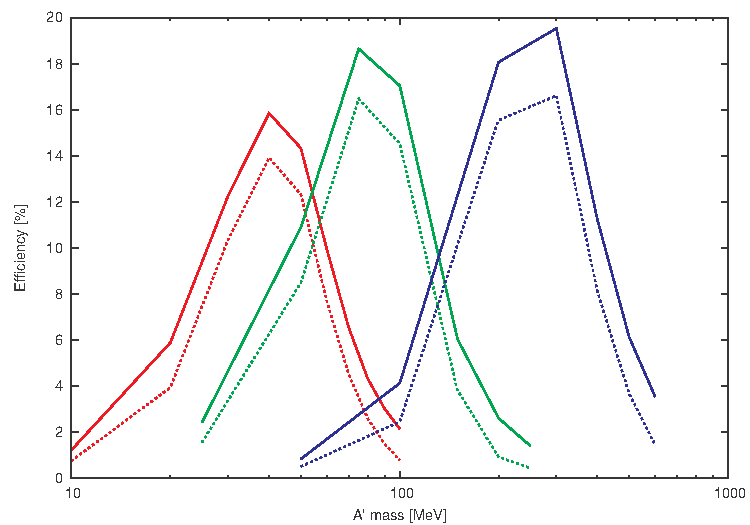
\includegraphics[width=\textwidth]{performance/trigger/ap_eff}
	\caption{\small{Trigger efficiency (solid lines) and combined efficiency (dashed lines) as a function of A' mass, at beam energies of 1.1, 2.2 and 6.6 GeV (red, green and blue respectively).}}
	\label{fig:trigeff}
\end{figure}

